\documentclass[12pt,a4paper]{article}
\usepackage[utf8]{inputenc}
\usepackage[T1]{fontenc}
\usepackage{graphicx}
\usepackage{amsmath}
\usepackage{amssymb}
\usepackage{empheq}
\usepackage{braket}
\usepackage[margin=1in]{geometry}

\usepackage{appendix}
\title{Linearized Gravity and QFT Connection}
\author{Matteo Falasca}
\date{March 2026}

\begin{document}
\maketitle

\begin{abstract}
In this work we present a modern and self‑contained review of the quantum theory of linearized gravity, starting from General Relativity and progressing to its canonical quantization. We then develop a minimal yet operational framework to describe gravitationally induced decoherence, deriving the master equation governing open quantum systems in the weak‑field regime.\end{abstract}

% ====================================================================
\section{Introduction to Linearized Gravity}
% ====================================================================

In GR, we speak of linearized gravity whenever our metric is almost flat. Technically, we can expand our metric around flat space:
\[
g_{\mu\nu} = \eta_{\mu\nu} + h_{\mu\nu}, \qquad |h_{\mu\nu}| \ll 1
\]
where $|h|$ is much smaller than 1.

\subsubsection*{Validity}

$h$ is different from observer to observer. Under an infinitesimal coordinate transformation, we have a family of diffeomorphisms of linearized metrics.
\[
h_{\mu\nu} \to h_{\mu\nu} + \partial_\mu \xi_\nu + \partial_\nu \xi_\mu, \qquad |\partial_\mu \xi_\nu| \ll 1
\]
The linearized metric behaves as a tensor under Lorentz transformations. In this sense, we can assume linearized gravity as Covariant, as long as we take slowly varying frame of reference compared to a valid one. \\
The complete diffeomorfism expansion around flat metric won't be much important for our calculations, but will be mathematically consistent in the next sections.

\subsection*{Equations of Motion}
Starting from the GR EoM
\[
R_{\mu\nu} - \frac{1}{2}g_{\mu\nu}R = 8\pi G\, T_{\mu\nu}
\]
it's first order terms in $h_{\mu\nu}$ are easily calculated by defining the trace and the trace-less perturbation:
\[
h = \eta^{\mu\nu} h_{\mu\nu}
\]
\[
\bar{h}_{\mu\nu} = h_{\mu\nu} - \frac{1}{2}\eta_{\mu\nu} h
\]
and then by computing the linearized Ricci and Einstein tensor:
\[
R_{\mu\nu}^{(1)} = \frac{1}{2}\left( -\Box h_{\mu\nu} - \partial_\mu \partial_\nu h + \partial^\lambda \partial_\mu h_{\nu\lambda} + \partial^\lambda \partial_\nu h_{\mu\lambda} \right)
\]
\[
G_{\mu\nu}^{(1)} = -\frac{1}{2}\left( \Box \bar{h}_{\mu\nu} + \eta_{\mu\nu} \partial^\lambda \partial^\rho \bar{h}_{\lambda\rho} - \partial^\lambda \partial_\mu \bar{h}_{\nu\lambda} - \partial^\lambda \partial_\nu \bar{h}_{\mu\lambda} \right)
\]

Due to diffeomorphism invariance, the metric perturbation contains redundant degrees of freedom. In 4D this reduces to 2 physical DoF in vacuum (gravitational waves), 6 with sources. This is well explained in Maggiore and confirmed by the Hamiltonian analysis in flat space via first-class constraints removing the unphysical modes.


 
\subsection*{Harmonic Gauge}

This gauge is covariant and expressed as:
\[
\boxed{\partial^\mu\bar{h}_{\mu\nu} = 0}
\]
We can always reach this gauge via a proper infinitesimal coordinate transformation:
\[
\partial^\mu \bar{h}_{\mu\nu} \to \partial^\mu \bar{h}_{\mu\nu} - \Box \xi_\nu
\]
In this gauge the Einstein equations reduce to:
\[
\Box \bar{h}_{\mu\nu} = \frac{-16\pi G}{c^4}\, T_{\mu\nu}
\]
which leads immediately to:
\[
\boxed{\partial^\mu T_{\mu\nu} = 0}
\]

\subsection*{TT Gauge}

In vacum, we can always find a Frame where \textsc{harmonic gauge holds and we can further impose:}
\begin{align}
    \Box \xi_{\mu\nu}=0 \quad \text{s.t.} \quad \xi_{\mu\nu} \equiv \partial_\mu\xi_\nu + \partial_\nu \xi_\mu -\eta_{\mu\nu}\partial_\rho\xi^\rho
\end{align}
This allows:
\begin{align}
\boxed{
    h^{0\mu}=0 \qquad h^i_i=0 \qquad \partial_i h^{ij}=0
}
\end{align}
In this framework the EoM are:
\[
\boxed{\Box h_{\mu\nu}=0}
\]
It is then straightforward to find a wave solution. Denoting by $(a,b)$ the plane perpendicular to the wave:
\[
h^{\mathrm{TT}}_{ij}(t,z) =
\begin{pmatrix}
h_+ & h_\times \\
h_\times & -h_+
\end{pmatrix}
\cos[\omega(t - z/c)]
\]






\section{Field Action}
In \textit{GR}, the \textit{covariance principle} requires the action to be invariant under coordinate changes. Since $\sqrt{-g}$ and $d^4x$ each produce a Jacobian factor under a change of coordinates, and the two cancel, covariance can be achieved by writing action in the form:
\[
S = \int d^4x \, \sqrt{-g}\, \bigl[ \mathcal{L}_{HE} + \mathcal{L}_M \bigr]
\]

We take $\mathcal{L}_{HE} = \frac{1}{16 \pi G} R$. Higher-curvature proposals exist, but we will not consider them here.

\subsection*{Linearized Gravity: Free action}

Linearized gravity is archieved expanding Hilbert-Einstein action around $g_{\mu\nu} \rightarrow \eta_{\mu\nu} + h_{\mu\nu}$. Action takes the form: 
\begin{align}
S^{(2)}_{HE}= -\frac{1}{64 \pi G} \int d^4x \bigl[
&\partial_\mu h_{\alpha\beta}\partial^\mu h^{\alpha\beta}
- \partial_\mu h \partial ^\mu h \nonumber \\
&+ 2\partial_\mu h^{\mu\nu}\partial_\nu h
-2\partial_\mu h^{\mu\nu}\partial_\rho h^\rho_\nu
\bigr]
\end{align}

Maggiore shows, form the unique action for a covariant massless and symmetric spin-2 field. Further orders are not relevant to our purposes: they complete the theory, but we would trace them out anyway. In the last chapter we show how they serve to reconstruct the full GR theory.

\vspace{0.5cm}
\subsection*{First gauge: Harmonic Gauge}
In canonical quantization is particurally simple to gauge theories. Covariance itself it's a gauge, as discussed initially. We will exploit this to get the harmonic Gauge, the analogue of the Feynmann gauge for QED, we do this by subtracting the
$\big(\partial^\nu\bar{h}_{\mu\nu}\big)^2$ zero. This is always feasible since under change of coordinates:
\[
\big( \partial^\nu\bar{h}_{\mu\nu} \big) ^2 \rightarrow
\big( \partial^\nu\bar{h}_{\mu\nu} - \square \xi_\mu\big) ^2
\]

Of cource, we have reduced the covariance of our action now, since we have chosen a class of frame of references. (QUESTION: in literature they chose whetever frame they want then go in TT gauge, is this really granted? I don't know) Our action now takes the form:
\begin{align}
\boxed{
S^{(2)}_{HE}= -\frac{1}{64 \pi G} \int d^4x \bigl[
-\partial_\mu h_{\alpha\beta}\partial^\mu h^{\alpha\beta}
+ \frac{1}{2}\partial_\mu h \partial ^\mu h
\bigr]}
\end{align}



\subsection*{Linearized action: Interaction terms}
We are interested in interaction between matter fields and linearized gravity. To analyse this in a simpler way, we will suppose that mass is described by a Klein-Gordon Lagrangian, because interaction structure is independent of the type of field we are using. Expanding the metric and its determinant into the matter part of the action, we will get a free matter contribute and various terms containing information about the gravity interacting with the matter:
\[
\int d^4x \,\sqrt{-g} \; \mathcal{L}_M
= S_M^{(0)} + S_M^{(1)} + S_M^{(2)} + \mathcal{O}(h^3)
\]

\textsc{HERE I JUST SHOW ALL CALCULATION:}\\
There are several approaches to compute this expansion, we take the most straightforward route and expand all terms in $S_M$ explicitly.

\vspace{0.5cm}


We begin by expanding the inverse metric:
\begin{align}
\boxed{
g^{\mu\nu}
= \eta^{\mu\nu}-h^{\mu\nu}+h^\mu_\alpha h^{\alpha\nu}
}\label{eq:g^}
\end{align}

which was calculated from an Ansatz and from asking $g^{\mu\alpha}g_{\mu\beta}=\delta^\alpha_\beta + \mathcal{O}(h^3)$.

\vspace{0.5em}

For the determinant factor:
\begin{align}
\boxed{
\sqrt{-g}
= 1 + \frac h2 + \frac14\bigl[\frac12h^2-h_{\alpha\beta}h^{\alpha\beta}\bigr]}
\label{eq:sqrt-g}
\end{align}

We have obtained it using '$\ln(\det(-g))=\text{tr} (\ln(-g))$' and
\[
\det g_{\mu\nu}
= \det\eta_{\mu\alpha}\det(\delta^\alpha_\nu+h^\alpha_\nu)
= (-1)\det(\mathbf{1+H})
\]

Then by expanding the logarithm and the exponential:
\[
-g= 1+h+\frac12\bigl(h^2-h^{ab}h_{ab}\bigr)
\]


\vspace{1em}
\textsc{\textbf{Interaction terms:}}
The zeroth-order term is, as expected, the free field action in flat space:
\[
\boxed{
S_M^{(0)}
= \int d^4x \Big(\frac{1}{2}\eta^{\mu\nu}\partial_\nu \phi \partial_\mu \phi - \frac{m^2}{2}\Big)}
\]

The first-order vertex couples $h_{\mu\nu}$ to the flat-space stress-energy tensor:
\[
\boxed {
S_M^{(1)} = -\frac12 \int d^4x \, h^{\mu\nu}T_{\mu\nu}
=
-\frac12 \int d^4x \, h^{\mu\nu}
\left[
\partial_\mu \phi\, \partial_\nu \phi
- \eta_{\mu\nu}\left(\frac12 \partial_\rho \phi\, \partial^\rho \phi + \frac12 m^2 \phi^2\right)
\right]
}
\]

The second-order vertex takes the form:
\begin{align}
\boxed{
S^{(2)}=\int d^4x \Biggl\{
\frac{1}{4}\bigl(\frac12h^2-h_{\alpha\beta}h^{\alpha\beta}\bigr)\mathcal{L}_M \nonumber - \frac{hh^{\mu\nu}}{4}\partial_\mu\phi\partial_\nu\phi \nonumber + \frac{1}{2}h^{\mu\alpha}h_\alpha^\nu \partial_\mu\phi\partial_\nu\phi
\Biggr\}
}
\end{align}

\textsc{Indexed are moved by the flat metric for convention}
\vspace{1cm}

 Of course, what we have constructed is a perturbative expansion of the theory. 
 In our Appendix we show that this perturbative theory can reconstruct all of GR, even if we intended graviton as a small perturbation of metric.

\section*{Action in TT gauge}
Simplifying more our action, since we will use these results to compute scattering matrixes, it is legit to keep only the DoF which survive on-shell condition and propagators by projecting with the TT projector. In the next chapter it will be obvious how we obtained this projector.\\

\vspace{0.5cm}
\textsc{Action terms in tt-gauge}\\

\boxed{
\begin{aligned}
S^{(2)}_{HE} &= \frac{1}{64 \pi G} \int d^4x \partial_k h_{ij}\partial^k h^{ij}
\\
S_M^{(0)} &= \int d^4x \Big(\frac{1}{2}\partial^i\phi \partial_i \phi - \frac{m^2}{2}\Big)\\
S_{I}^{(1)} &= -\frac{1}{2}\int d^4x\; h^{ij}\,\partial_i\phi\,\partial_j\phi\\
S^{(2)}_{I} &= \int d^4x \Biggl[
\frac{1}{4} h_{\alpha\beta}h^{\alpha\beta}
\left( \frac{1}{2}\partial_\rho\phi\partial^\rho\phi
- \frac{1}{2}m^2\phi^2 \right)
+ \frac{1}{2} h^{\mu\alpha}h_{\alpha}^{\nu}
\partial_\mu\phi\partial_\nu\phi
\Biggr] \\[6pt]
\end{aligned}
}\\

Where the projector is:
\[
\Lambda_{ij,kl}(\hat{n}) = \frac{1}{2}\left(P_{ik}P_{jl} + P_{il}P_{jk} - P_{ij}P_{kl}\right)
\]
and:
\[
P_{ij}=\delta_{ij}-n_in_j
\]

% ====================================================================
\section{Interaction Hamiltonian}
% ====================================================================

Since we are in a perturbation theory, we can go into interaction picture. In the interaction picture:
\[
\hat{H} = \hat{H}_0^{\mathrm{KG}} + \hat{H}_0^{\mathrm{PF}} + \hat{H}^I
\]




The Hamiltonian densities in the interaction picture are:
\begin{align}
    \mathcal{H}_0^{\mathrm{KG}} &= \pi_\phi \dot\phi - \mathcal{L}_{\mathrm{KG}} = \frac{1}{2}\Bigl(\pi_{\phi}^2 + (\vec{\nabla}\phi)^2 - \frac12m^2\phi^2\Bigr) \\
    \mathcal{H}_0^{\mathrm{PF}} &= \pi_h^{\alpha \beta} \dot h_{\alpha \beta} - \mathcal{L}_0^{PF} = \frac{1}{2\kappa^2}\Bigl(\pi_{\mu\nu}^{\ }\pi^{\mu\nu} + (\vec{\nabla}h_{\mu\nu})\cdot(\vec{\nabla}h^{\mu\nu})\Bigr)
\end{align}

\texttt{Conjugate momenta}, at first and second order:
\begin{equation}
    \Pi_\phi ^{(1)}= 0
\end{equation}

\begin{equation}
\Pi_\phi ^{(2)} = \frac{1}{4} h_{\alpha\beta}h^{\alpha\beta}\partial^0\phi
\end{equation}

The full Hamiltonian is:
\begin{align}
    \mathcal{H} &= \frac{1}{2}\Bigl(\pi_\phi^2 + (\vec{\nabla}\phi)^2 - \frac12m^2\phi^2 \Bigr)+ \frac{1}{2\kappa^2}\Bigl(\pi_{\mu\nu}^{\ }\pi^{\mu\nu} + (\vec{\nabla}h_{\mu\nu})\cdot(\vec{\nabla}h^{\mu\nu})\Bigr) \notag\\
    & \quad+ \frac12\, h_{ij} \Bigl(\partial^i\phi\,\partial^j\phi \Bigr)  \\ &  \quad+ \frac{1}{4} h_{\alpha\beta}h^{\alpha\beta} \left( \frac{1}{2} \partial^0\phi \partial_0\phi + (\nabla^2\phi)^2 - \frac{1}{2}m^2\phi^2 \right) + \frac{1}{2} h^{\mu\alpha}h_{\alpha}^{\nu} \partial_\mu\phi\partial_\nu\phi 
\end{align}

We may explicit the perturbative nature of this theory by making the transformation $h \rightarrow \kappa  h$, then:
\begin{align}
    \boxed{
    \mathcal{H}_I= \frac{\kappa}2\, h_{ij} \Bigl(\partial^i\phi\,\partial^j\phi \Bigr) + \frac{\kappa^2}{4} h_{\alpha\beta}h^{\alpha\beta} \left( \frac{1}{2} \partial^0\phi \partial_0\phi + (\nabla^2\phi)^2 - \frac{1}{2}m^2\phi^2 \right) + \frac{\kappa^2}{2} h^{\mu\alpha}h_{\alpha}^{\nu} \partial_\mu\phi\partial_\nu\phi}
\end{align}

Again, we notice that this is very similar to scalar QED, where the interacting Hamiltonian has quadratic term in the boson field.


\section{Field Quantization of Free Theory}


We follow the canonical quantization procedure: write the Fourier expansion of the field and promote the mode coefficients to creation and annihilation operators asking for ETCR. Let's just notice that the diffeomorfism that allows the TT gauge is linear, i.e. it can be summed upon multiple waves. Let's just remember canonical quantization is done on normalized cinetical terms, so what we are expressing now is the canonical h field:

\begin{equation}
\boxed{
    \hat{h}_{\mu\nu} = \int \frac{d^3k}{\sqrt{(2\pi)^3 2\omega_k}}
    \sum_{\lambda=+,\times}
    \Bigl(
        \hat{a}_{\vec{k},\lambda}\, e^{-ik\cdot x}\, \epsilon_{\mu\nu}(\lambda,k)
        +
        \hat{a}^{\dagger}_{\vec{k},\lambda}\, e^{+ik\cdot x}\, \epsilon_{\mu\nu}(\lambda,k)
    \Bigr)
}
\end{equation}

\subsection*{Polarization vectors and TT-projector}
We recover from classical solutions, the orthonormal basis of the spin-2 space, orthogonal to the direction of the wave $n$. Expressed with respect to the orthonormal basis $\{u_i, v_i, n_i\}$.

\[
\epsilon^{(+)}_{\mu\nu} = \frac{1}{\sqrt{2}}
\left( u_\mu u_\nu - v_\mu v_\nu \right)
\]

\[
\epsilon^{(\times)}_{\mu\nu} = \frac{1}{\sqrt{2}}
\left( u_\mu v_\nu + v_\mu u_\nu \right)
\]

\texttt{PROJECTORS}\\
We can recover their useful projector by noticing that the spatial identity decomposes as $
\delta_{ij} = u_i u_j + v_i v_j + n_i n_j $, so the transverse projector is 
$P_{ij} = \delta_{ij} - n_i n_j = u_i u_j + v_i v_j$,
which projects onto the plane orthogonal to $\hat{n}$.

The sum over physical polarization states defines the rank-4 tensor
\[
\Lambda_{ij,kl} = \sum_{A=+,\times} \epsilon^A_{ij}\epsilon^A_{kl}.
\]
Using the explicit forms of $\epsilon^{(+)}_{ij}$ and $\epsilon^{(\times)}_{ij}$ and the properties of $P_{ij}$, one obtains after straightforward algebra and symmetrization:
\[
\boxed{
\Lambda_{ij,kl}(\hat{n}) = \frac{1}{2}\left(P_{ik}P_{jl} + P_{il}P_{jk} - P_{ij}P_{kl}\right).
}
\]

This tensor is the projector onto the space of symmetric, transverse and traceless rank-2 tensors, and it satisfies
\[
\Lambda_{ij,kl} T_{kl} = T^{TT}_{ij}.
\]
\subsection*{Commutation Relations}

Imposing equal-time canonical relations (ETCR):
\begin{equation}
    \bigl[\hat{h}_{\mu\nu}(x_1,t),\, \hat{\pi}_{\alpha\beta}(x_2,t)\bigr]
    = i\,\delta^{(3)}(\vec{x}_1 - \vec{x}_2)\, \delta^{\mu\nu}_{\;\;\alpha\beta}
\end{equation}
with conjugate momentum:
\begin{equation}
    \hat{\pi}_{\mu\nu} = -\partial_0 \hat{h}_{\mu\nu}
\end{equation}
we recover the canonical second-quantization structure:
\begin{equation}
      \bigl[\hat{a}_{\mathbf{k},\lambda},\, \hat{a}^{\dagger}_{\mathbf{k}',\lambda'}\bigr] = \delta^{\lambda}_{\lambda'} \delta^{(3)}(\mathbf{k}-\mathbf{k}')
\end{equation}

\subsection*{Derivation of $\bigl[\hat{a}_{\mathbf{k},\lambda},\,\hat{a}^{\dagger}_{\mathbf{k}',\lambda'}\bigr]$}

To prove the canonical structure, introduce the tensor scalar product:
\begin{equation}
    \langle A, B \rangle = i\int d^3x \, A^*_{\mu\nu}(x) \overset{\leftrightarrow}{\partial_0} B^{\mu\nu}(x)
\end{equation}
where $A \overset{\leftrightarrow}{\partial_0} B \equiv A(\partial_0 B) - (\partial_0 A) B$. When we use this on single oscillation modes and the field itself we have:
\begin{align}
    \langle h(\vec{k},\lambda),\, h(\vec{k}',x) \rangle &= \delta_{\lambda \lambda'} \delta^{(3)}(\mathbf{k}-\mathbf{k}') \\
    \langle h(\vec{k},\lambda),\, h^{*}(\vec{k}',x) \rangle &= 0
\end{align}
and consequently:
\begin{align}
    \langle\hat{h}(\vec{k},\lambda),\, \hat{h}(\vec{x})\rangle &= \hat{a}_{k,\lambda} \\
    \langle\hat{h}^*(\vec{k},\lambda),\, \hat{h}(\vec{x})\rangle &= -\hat{a}^{\dagger}_{\vec{k},\lambda}
\end{align}
The explicit form of the operators is:
\begin{equation}
    \hat{a}^{\dagger}_{\vec{k},\lambda} = i \int \frac{d^3x}{\sqrt{(2\pi)^3 2\omega_k}} \; e^{ik\cdot x}\, \varepsilon^{\mu\nu}(\mu,\lambda) \Bigl(\hat{\pi}_{\mu\nu} - i\omega_k \hat{h}_{\mu\nu}(x)\Bigr)
\end{equation}
\begin{equation}
    \hat{a}^{\dagger}_{\vec{k},\lambda} = -i \int \frac{d^3x}{\sqrt{(2\pi)^3 2\omega_k}} \; e^{ik\cdot x}\, \varepsilon^{\mu\nu}(k,\lambda) \Bigl(\hat{\pi}_{\mu\nu}(x) + i\omega_k \hat{h}_{\mu\nu}(x)\Bigr)
\end{equation}
Computing the commutator via the ETCR and the mode expansion:
\begin{align}
    \bigl[\hat{a}_{k,\lambda},\, \hat{a}^{\dagger}_{k',\lambda'}\bigr]
    &= (-i) i \int \frac{d^3x\, d^3x'}{(2\pi)^3 \sqrt{4\omega_k\omega_{k'}}} \; e^{i(k\cdot x - k'\cdot x')} \; \epsilon^{\mu\nu}(k,\lambda)\, \epsilon^{\rho\sigma}(k',\lambda') \notag\\
    &\quad \times \Bigl(\hat{\pi}_{\mu\nu} - i\omega_k \hat{h}_{\mu\nu}\Bigr) \Bigl(\hat{\pi}_{\rho\sigma} + i\omega' \hat{h}_{\rho\sigma}\Bigr) \\
    &= \int \frac{d^3x\, d^3x'}{(2\pi)^3 \sqrt{4\omega_k\omega_{k'}}} \; e^{i(k-k')\cdot x} \; \epsilon^{\mu\nu}\, \epsilon^{\mu\nu} \left[ -i\omega_k\, \delta^{(3)}(\vec{x}-\vec{x}') + i\omega_{k'}\, \delta^{(3)}(\vec{x}-\vec{x}') \right]
\end{align}
\begin{equation}
    \boxed{ \bigl[\hat{a}_{k,\lambda},\, \hat{a}^{\dagger}_{k',\lambda'}\bigr] = \delta_\lambda^{\;\lambda'}\,\delta^{(3)}(\vec{k}-\vec{k}') }
\end{equation}
% ====================================================================
\section{Feynman Propagators}
% ====================================================================
The Feynman propagator in the Transverse-Traceless (TT) gauge describes the propagation of the two physical degrees of freedom of the graviton. It is defined as:
\begin{align}
    i D_{F, \text{TT}}^{ij,kl}(x-y) &= \langle 0 \mid T\bigl[\hat{h}_{TT}^{ij}(x)\,\hat{h}_{TT}^{kl}(y)\bigr] \mid 0\rangle \notag\\
    &= \int \frac{d^3k}{(2\pi)^3 2\omega_k} \;\sum_{\lambda=+, \times} \epsilon^{ij}(\mathbf{k},\lambda)\,\epsilon^{kl}(\mathbf{k},\lambda) \notag\\
    &\quad \times \Bigl( \Theta(x_0 - y_0)\,e^{-ik(x-y)} + \Theta(y_0 - x_0)\,e^{ik(x-y)} \Bigr)
    \\=&
\int \frac{d^3k}{(2\pi)^3\,2\omega_k}
\sum_{\lambda=+,\times}
\epsilon^{ij}(\mathbf{k},\lambda)\epsilon^{kl}(\mathbf{k},\lambda) \notag 
\int \frac{dk^0}{2\pi}\;
\frac{i\,e^{-ik\cdot(x-y)}}{(k^0)^2-\omega_k^2+i\epsilon} \\=&\int \frac{d^4k}{(2\pi)^4}\;
\frac{i\,P^{ij,kl}(\mathbf{k})}{\textbf{k}^2+i\epsilon}\;
e^{-ik\cdot(x-y)}
\end{align}

Where we used the projection of the polarization vectors:
\begin{equation}
    \sum_{\lambda=+, \times} \epsilon_{ij}(\mathbf{k},\lambda)\,\epsilon_{kl}(\mathbf{k},\lambda) = \frac{1}{2}\Bigl(P_{ik}P_{jl} + P_{il}P_{jk} - P_{ij}P_{kl}\Bigr) \equiv \Lambda_{ij,kl}(\hat{k})
\end{equation}

Finally, our propagator regards only spatial components:
\begin{equation}
    \boxed{ D_{F, \text{TT}}^{ij,kl}(k) = \frac{\Lambda^{ij,kl}(\hat{k})}{k^2  + i\varepsilon} }
\end{equation}
Unlike the De Donder gauge propagator, this form is not manifestly Lorentz covariant due to the explicit dependence on the propagation direction $\hat{k}$, but it correctly isolates the radiative degrees of freedom $h_{ij}^{(+)}$ and $h_{ij}^{(\times)}$.



% ====================================================================
\section{S-Matrix}
% ====================================================================

With the Hamiltonian density in the interaction picture, the scattering matrix at the required order in $\kappa$ is:
\begin{equation}
    \hat{S} = \hat{U}(-\infty,+\infty) = \sum_{n=0}^{\infty} \frac{1}{n!}\,(-i)^n \int d^4x_1 \cdots d^4x_n\; T\!\Bigl(\hat{\mathcal{H}}_I(t_1)\cdots\hat{\mathcal{H}}_I(t_n)\Bigr)
\end{equation}

We keep at most second order in $\kappa$ interactions:
\begin{align}
\hat{S}^{(1)} = &-i \Bigg\{ 
 \frac{\kappa}{2} \int d^4x \; :h_{ij}\, \partial^i \phi \, \partial^j \phi: \notag\\
& + \frac{\kappa^2}{4} \int d^4x \; :h_{\alpha\beta} h^{\alpha\beta}
\left( \frac{1}{2}\partial^0\phi\,\partial_0\phi
+ \frac{1}{2}(\nabla \phi)^2
+ \frac{1}{2} m^2 \phi^2 \right): \notag\\
& + \frac{\kappa^2}{2} \int d^4x \; :h^{\mu\alpha} h_{\alpha}^{\ \nu}
\, \partial_\mu \phi \, \partial_\nu \phi:
\Bigg\} \\
\\
\hat{S}^{(2)} =
& -\frac{\kappa ^ 2}{8}\int d^4x_1\, d^4x_2 \; :
h^{ij}(x_1)\partial_i \phi(x_1)\partial_j \phi(x_1)\,
h^{kl}(x_2)\partial_k \phi(x_2)\partial_l \phi(x_2):
\end{align}

\section*{Scalar--Scalar Interaction in the Non-Relativistic Limit}
Let's start to study the behaviour of this theory, our first result is that in the non relativistic limit, gravitons don't mediate any force. In fact, from Wick's theorem, the only contribute from scalar--scalar interaction will be:
\begin{equation}
  S_{fi} = \Bra{k_1,\, k_2}\, \hat{S}^{(2)} \,\Ket{k_3,\, k_4}
\end{equation}

However let's remember that in the Non Relativistic limit, we have $
p^\mu=(m,0,0,0) + O(v) $.
Since our projector involves only spatial components of the 4-moments, this scattering matrix element will be zero. 
Even if we alredy know, let's just see how we shall proceed for the next calculations:
\begin{align*}
S_{fi} &= \bra{0}\hat{a}_{k_1}\hat{a}_{k_2} \;
 \left\{-\frac{1}{8}s \int dx_1\, dx_2 \;
i D_F(x_1 - x_2)
\right. \notag \\
&\quad \times \int d^3 q_1\, d^3 q_2\, d^3 q_3\, d^3 q_4
\;
\frac{1}{4\sqrt{E_{q_1}\, E_{q_2}\, E_{q_3}\, E_{q_4}}(2\pi)^6}
\\
&\qquad \times :
\partial_\mu\!\left(e^{-iq_1\cdot x_1}\hat{a}_{q_1}
+ e^{+iq_1\cdot x_1}\hat{a}^\dagger_{q_1}\right)
\\
&\qquad \times \partial_\nu\!\left(e^{-iq_2\cdot x_2}\hat{a}_{q_2}
+ e^{+iq_2\cdot x_2}\hat{a}^\dagger_{q_2}\right)
\\
&\qquad \times \partial_\rho\!\left(e^{-iq_3\cdot x_1}\hat{a}_{q_3}
+ e^{+iq_3\cdot x_1}\hat{a}^\dagger_{q_3}\right)
\\
&\qquad \times \partial_\sigma\!\left(e^{-iq_4\cdot x_2}\hat{a}_{q_4}
+ e^{+iq_4\cdot x_2}\hat{a}^\dagger_{q_4}\right)
: \biggr\}
\hat{a}^\dagger_{k_3}\hat{a}^\dagger_{k_4}\ket{0}
\end{align*}

All terms have the same form, but they contain the projection on space components of the 4-momentums, which have just time component, therefore everything is zero:

\begin{align} 
S_{12/34} & \propto -\frac{i}{16} \int \frac{d^3q_1 d^3q_2 d^3q_3 d^3q_4}{(2\pi)^6 \sqrt{16E_1E_2E_3E_4}} \int d^4x_1 d^4x_2 \int \frac{d^4 q}{(2\pi)^4} \widetilde{D}_F(q) e^{-iq\cdot(x_1-x_2)} \nonumber \\
& \quad \times \Lambda^{\mu\nu\rho\sigma} q_{1\mu} q_{2\nu} q_{3\rho} q_{4\sigma} e^{i(q_1+q_2)\cdot x_1} e^{-i(q_3+q_4)\cdot x_2} \bra{k_1k_2}\hat{a}_{q_1}^\dagger\hat{a}_{q_2}^\dagger\hat{a}_{q_3}\hat{a}_{q_4}\ket{k_3k_4} \\
&\simeq 0
\end{align}

Our total Scattering amplitude is:

\begin{align}
\boxed{
    S_{fi,TOT}=0 + \mathcal{O}(v)}
\end{align}

\subsection*{Compton Scattering}
\subsubsection*{First-order Scattering matrix (SEAGULL TERMS)}
\begin{align}
\langle k_1, k_2, \lambda_2 \,|\, \hat{S}^{(1)} \,|\, k_3, k_4 \lambda_4 \rangle
= - i\kappa^2 \int d^4x \;\langle k_1, k_2\lambda_2 \,|\,
{:} &[-\frac18 h_{\alpha\beta} h^{\alpha\beta}
\!\left((\partial_0 \phi)^2+(\nabla\phi)^2 - m^2\phi^2\right)
\\& + \frac{1}{2} h^{\mu\alpha} h^\nu_\alpha   \partial_\mu\phi \partial_\nu\phi]
{:}\,|\, k_3, k_4 \lambda_4 \rangle
\notag\\
\end{align}
\begin{align}
\,\,\,\,\,\,\,\,\,\, = -i\kappa^2 &\int \frac{d^4x}{(2\pi)^4} \;\langle k_1, k_2\lambda_2 \,|\;
\int \frac{d^3q_1 d^3q_2 d^3q_3 d^3q_4}{(2\pi)^2\sqrt{16E_1\cdots E_4}}\;
\Bigg[-\frac18
\!\left(e^{-iq_2 x}\epsilon_{\alpha\beta}\hat{a}_{q_2\lambda_2}+\text{h.c.}\right)
\\
&\left(e^{-iq_4 x}\epsilon '^{\alpha\beta}\hat{a}_{q_4\lambda_4}+\text{h.c.}\right)\times \left(-q^0_1q_3^0-\vec{q_1}\cdot \vec{q_3}+m^2\right) |k_3, k_4\lambda_4\rangle\\
&= i\kappa ^2 \frac{\delta^{(4)(K_{in}-K_{out})}}{(2\pi)^2\sqrt{16E_1E_2E_3E_4}}\Bigl(\frac{\epsilon^{(2)}\cdot\epsilon^{(4)}}{2}
(-k_1^0k_3^0-\vec{k_1}\cdot\vec{k_3}+m^2)+(\epsilon_{(2)}^{\mu\alpha}\epsilon_{(4)\alpha}^\nu k_{1\nu}k_{3\mu})\Bigr)
\end{align} 

\subsubsection*{Second-order Scattering Matrix}
The second-order S-matrix gives the contribution:
\begin{equation}
    \hat{S}^{(2)} = -\frac{1}{2} \int d^4x_1\, d^4x_2\; {:}\,\mathcal{H}_I(x_1)\,\mathcal{H}_I(x_2)\,{:}
\end{equation}

And its matrix element is:

\begin{align*}
S_{fi}
&= \langle k_1 ,k_2 \lambda_2 \mid \hat{S}^{(2)} \mid k_3,k_4\lambda_4\rangle \notag\\
&=  (-\frac{\kappa^4}{8}) \langle 0 \mid \hat{a}_{k_1} \hat{a}_{k_2,\lambda_2}
\int d^4x\, d^4x'\;\;
{:}
h_{\mu\nu}(x)\partial^\mu\phi(x)\partial^\nu\phi(x){:}
\;
{:}h_{\rho\sigma}(x')\partial^\rho\phi(x')\partial^\sigma\phi(x'){:}\;
\hat{a}^{\dagger}_{k_3}\hat{a}^{\dagger}_{k_4,\lambda_4}
\mid 0\rangle 
\end{align*}

Due to Wick theorem on time ordering and to graviton simmetry, we have 4 identical contributes. We then call q the moment going through the propagator and expand into modes:

\begin{align*}
&= -4\frac{\kappa^2}{8}\, i
\bra{0} \hat{a}_{k_1} \hat{a}_{k_2,\lambda_2}
\partial^\mu_{x_1}\partial^\rho_{x_2} \int d^4x_1 d^4 x_2 \, D_F(x_1-x_2)
:\hat{h}_{\mu\nu}(x_1)\hat{h}_{\rho\sigma}(x_2)
\partial^\nu_{x_1}\partial^\sigma_{x_2}
\hat{\phi}(x_1)\hat{\phi}(x_2):
\hat{a}^{\dagger}_{k_3}\hat{a}^{\dagger}_{k_4,\lambda_4}
\ket{0} \\
&= -i\frac{\kappa^4}{2}
\int d^4x_1 d^4x_2
\int d^3q_1 d^3q_2 d^3q_3 d^3q_4
\int \frac{d^4q}{(2\pi)^4}
\sum_{\lambda,\lambda'}^{+,\times}
\sqrt{
\frac{1}{(2\pi)^3 2E_{q_1}
(2\pi)^3 2E_{q_2}
(2\pi)^3 2E_{q_3}
(2\pi)^3 2E_{q_4}}
} \\
&\quad \times
\bra{0}\hat{a}_{k_1} \hat{a}_{k_2,\lambda_2}
\frac{e^{-iq(x_1-x_2)}}{q^2 - m^2 + i\varepsilon}
 q^\mu q^\rho q_1^\nu q_3^\sigma \\
&\quad \times
\Bigl\{
\bigl(
e^{iq_2 x_1}\epsilon_{\mu\nu}(q_2,\lambda)\hat{a}^\dagger_{q_2,\lambda}
\,e^{-iq_4 x_2}\epsilon_{\rho\sigma}(q_4,\lambda')\hat{a}_{q_4,\lambda'}
+ \text{h.c.}
\bigr) \\
&\qquad \times
\bigl(
e^{iq_1 x_1}\hat{a}^\dagger_{q_1}
\,e^{-iq_3 x_2}\hat{a}_{q_3}
+ \text{h.c.}
\bigr)
\Bigr\}
\hat{a}^{\dagger}_{k_3}\hat{a}^{\dagger}_{k_4,\lambda_4}
\mid 0\rangle \\
\end{align*}

Now, we have use the properties of the creation and annihilation operators. Furthermore, we use the integrals over space to explicitly describe two Dirac Delta functions. 

\begin{align*}
&= -\frac{i\kappa^2}{2}\int \frac{d^4q}{(2\pi)^4}
\int \frac{d^4q_1\,d^3q_2\, d^3q_3\, d^3q_4}{(2\pi)^6 \sqrt{16 E_1E_2E_3 E_4}}
\frac{q^{\mu}q^{\rho}q_1^{\nu}{q}^\sigma_{3}}{q^2 - m^2 +i\varepsilon}
\epsilon_{\mu\nu}^{(2)}\epsilon_{\rho\sigma}^{(4)}
\nonumber\\
&\quad \times (2\pi)^8
\Biggl\{
\delta^{(4)}(q_1+q_2-q)\,\delta^{(4)}(q_3+q_4-q)\;
\delta^{\lambda_4}_{\lambda'} \, \delta^{\lambda_2}_{\lambda} \delta^{k_2}_{q_2}\delta^{k_1}_{q_1}\delta^{k_3}_{q_3}\delta^{k_4}_{q_4} \\
&\quad
+\,\delta^{(4)}(q_2-q_1-q)\,\delta^{(4)}(q_3-q_4+q)\;
\delta^{\lambda_4}_{\lambda'} \, \delta^{\lambda_2}_{\lambda} \delta^{k_2}_{q_2}\delta^{k_1}_{q_3}\delta^{k_3}_{q_1}\delta^{k_4}_{q_4} \\ \\
&\qquad
+\,\delta^{(4)}(-q_2+q_1-q)\,\delta^{(4)}(q_4-q_3+q)\;
\delta^{\lambda_4}_{\lambda} \, \delta^{\lambda_2}_{\lambda'} \delta^{k_2}_{q_4}\delta^{k_1}_{q_1}\delta^{k_3}_{q_3}\delta^{k_4}_{q_2} \\\\
&\qquad
+\,\delta^{(4)}(-q_2-q_1-q)\,\delta^{(4)}(q_4+q_3+q)\;
\delta^{\lambda_4}_{\lambda} \, \delta^{\lambda_2}_{\lambda'} \delta^{k_2}_{q_4}\delta^{k_1}_{q_3}\delta^{k_3}_{q_1}\delta^{k_4}_{q_2}
\Biggr\}
\end{align*}
Where we omitted that $\delta^q_k=\delta^{(3)}(q-k)$. There are two identical contributions. Since we have scalar products, it's legit to go to the frame where $\vec{k}_{i,\mathrm{tot}}=0$. Hiding the delta:
\begin{align*}
&= -\frac{i\kappa^2}{(2\pi)^2\sqrt{16E_1 E_2 E_3 E_4}}
\\
&\quad \times
\Biggl\{
D_F(k_1+k_2)\;k_1^\mu k_1^\nu
k_3^\rho k_3^\sigma\,
\epsilon_{\mu\nu}(k_2,\lambda_2)\epsilon_{\rho\sigma}(k_4,\lambda_4)
\nonumber\\
&\qquad
+\,D_F(k_3-k_2)\;k_3^\mu k_3^\nu
k_1^\rho k_1^\sigma\,
\epsilon_{\mu\nu}(k_2,\lambda_2)\epsilon_{\rho\sigma}(k_4,\lambda_4)
\nonumber\Biggr\}
\end{align*}
From the polarization tensor rules, since we could always go into a frame of reference where the scalar is resting $(m,0,0,0)$, and because the polarization tensor has got no other contributes other than space-like ones. It all goes to zero:

\begin{align}
S_{fi}
&= -i \kappa^2
\frac{\delta^{(4)}(k_1-k_2+k_3-k_4)}{(2\pi)^2 \sqrt{16 E_1 E_2 E_3 E_4}}
\frac{1}{(k_3 - k_2)^2 - m^2 + i\epsilon}
\nonumber
k_3^\mu k_3^\nu\,
\epsilon_{\mu\nu}^{(2)}
\,k_1^\rho k_1^\sigma\,
\epsilon_{\rho\sigma}^{(4)}=0
\end{align}

The full scattering amplitude is then:

\begin{empheq}[box=\fbox]{align}
    S_{fi}&= i\kappa ^2 \frac{\delta^{(4)(K_{in}-K_{out})}}{(2\pi)^2\sqrt{16E_1E_2E_3E_4}}\Bigl(\frac{-1}{(k_3-k_2)^2-m^2+i\epsilon}k^\mu_3 k^\nu_3\epsilon_{\mu\nu}^{(2)}k_1^\rho k_1^\sigma \epsilon_{\rho\sigma}^{(4)}+\\&    \frac{\epsilon^{(2)}\cdot\epsilon^{(4)}}{2}
(-k_1^0k_3^0-\vec{k_1}\cdot\vec{k_3}+m^2)+(\epsilon_{(2)}^{\mu\alpha}\epsilon_{(4)\alpha}^\nu k_{1\nu}k_{3\mu})\Bigr)
\end{empheq}

\section{Scattering Amplitude}
We will compute scattering cross section, by considering a scalar still in the laboratory frame, or equivalently in the non-relativistic limit. Our computation will follow Greiner's one. So we will consider the cross section in the limit where the ingoing current is just a particle entering in the infinitesimal box. What we will see is that, due to the graviton momentum scalar product in the amplitude, we get processes which prefer the backward scattering.

\begin{equation}
    d \sigma = \int |S_{fi}|^2 \frac{1}{J_{in}} \frac{Vd^3p_3}{(2\pi)^3}\frac{Vd^3p_4}{(2\pi)^3}
\end{equation}



This espression simplifies a lot due to our hypothesis. We have only one contirbute from the scattering matrix elements, since the time part of the polarization vectors is zero, so they can't be contracted with the ingoing scalar 4-momentum. Moreover, we will use the following substitution $\frac{d^3p_3}{2E}=\int d^4p_3 \delta^{(4)}(p^2-m^2)\Theta(p_0)$. What we get is:

\begin{align}
d\sigma
&=
\frac{k^4}{(2\pi)^4 }
\int d^3p_3d^3p_4 \delta^{(4)}\!\left(K_{\mathrm{out}}-K_{\mathrm{in}}\right)\,
\frac{(2\pi)^2}{16\,\omega_2 m}
\,
\frac{1}{\omega_4E3}
\,
\left|\epsilon_4\!\cdot\!\epsilon_2\right|^2
\,
\frac{(m E_3 - m^2)^2}{4} 
\\&
=
\frac{k^4}{(2\pi)^4 }
\frac{2(2\pi)^2}{64\omega_2}
\int d|p_3| d\Omega_3\, d^3p_4\;
\delta^{(4)}\!\left(K_{\mathrm{out}}-K_{\mathrm{in}}\right)
\,
\left|\epsilon_4\!\cdot\!\epsilon_2\right|^2
\,
\frac{m\,(E_3 - m)^2|\vec p_4|}{2E_3}


\end{align}
Let's just remember that our volume in the continuous case is just $(2\pi)^3$.
Now we use that, after some simple computation, where we have at most used the rul for the dirac delta of a function:
\begin{align}
&\int_0^\infty |\vec{p_4}d|\vec{p_4}| \int\frac{md^3p_3}{2E_3}\delta^{(4)}(K_{out}-K_{in})|E_3-m|^2=\frac{\omega_4^2}{2\omega_2}(\omega_4-\omega_2)^2
\end{align}
And from the delta used in the integral we get the ususal formula for the scattered energy:

\begin{equation}
    \omega_4 = \frac{\omega_2}{1+\frac{\omega_2}{m}(1-cos\,\theta)}
\end{equation}

By using the evaluation of this integral into our scattering cross section we have an expression which is coherent with the unity of measure $E^{-2}$:

\begin{equation}
    \frac{d\sigma}{d\Omega_3}=4G^2\frac{\omega_4^4}{\omega_2^2}(\omega_4-\omega_2)^2 |\epsilon_4 \cdot \epsilon_2|^2
\end{equation}

Of course we will take the average over incoming states and the sum over outgoing ones for this quantity, so the cross section is summed over all helicities and divided by 4.

We are interested in evaluating the polarization sums appearing in scalar products of polarization vectors. This can be done by explicitly using their geometric construction. The polarization vectors $\epsilon$ live in the transverse plane orthogonal to the spatial momentum and can be expressed as linear combinations of two real orthonormal vectors $u$ and $v$, with
\[
u \cdot v = 0, \qquad u^2 = v^2 = 1.
\]

If we consider two different momenta $k_2$ and $k_4$, we choose the transverse bases such that the plane defined by $k_2$ and $k_4$ is aligned with that defined by $u_2$ and $u_4$. With this choice, the relevant scalar products reduce to
\begin{align}
   u_2 \cdot u_4 &= \cos \theta,\\
   v_2 \cdot v_4 &= 1,\\
   u_2 \cdot v_4 &= v_2 \cdot u_4 = 0.
\end{align}

what we get is:

\begin{align}
    &\epsilon (k_2,+)\cdot \epsilon (k_4, +) = \frac12(cos^2\theta+1)\\
    &\epsilon (k_2,+)\cdot \epsilon (k_4, \times) = 0\\
    &\epsilon (k_2,+)\cdot \epsilon (k_4, +) = cos\, \theta
\end{align}

Finally, we have 
$$
\boxed{
\frac{d\sigma}{d\Omega_3}=G^2(cos^4\theta + 6 cos ^ 2\theta+1 )\frac{\omega_4^4}{\omega_2^2}(\omega_4-\omega_2)^2 
}
$$

Its behaviour it's completely different from those from Scalar QED Compton scattering, mostly because of the cinetic term in the lagrangian and because the graviton has spin 2.

\begin{center}
    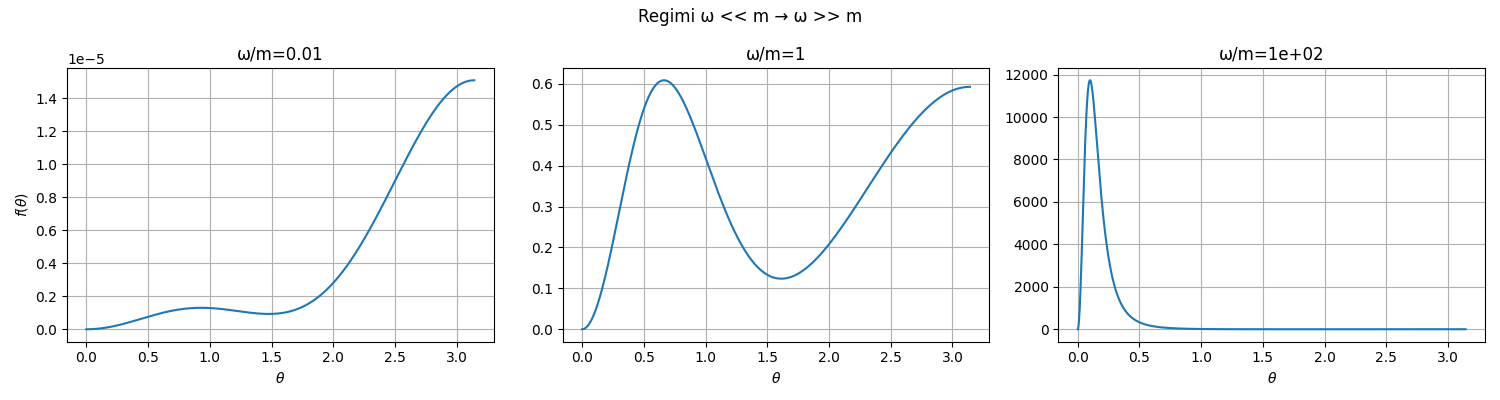
\includegraphics[width=16cm]{dsigma2.png}
\end{center}
% ====================================================================
\appendix
\section{Full linearized theory}
% ====================================================================

Expanding the Einstein–Hilbert action around a flat background generates an infinite 
series of nonlinear self–interaction terms for the gravitational field. At linear order, 
the equations of motion take the form


\[
\mathcal{E}_{\mu\nu}^{\alpha\beta} h_{\alpha\beta}
= \frac{\kappa}{2} T_{\mu\nu},
\]


where \(\mathcal{E}_{\mu\nu}^{\alpha\beta}\) denotes the linearized Einstein operator.

With the allowed gauges, matter fields satisfy


\[
\partial^\mu T_{\mu\nu} = 0,
\]
However, expanding higher orders in \(\kappa\), the gravitational field contributes to its own source. 
The equations of motion can be written schematically as
\begin{equation}
\mathcal{E}_{\mu\nu}^{\alpha\beta} h_{\alpha\beta}
= \frac{\kappa}{2}\left( T_{\mu\nu} + t_{\mu\nu}[h] \right),
\end{equation}
where \(t_{\mu\nu}[h]\) is the energy–momentum pseudotensor arising from the nonlinearities of the Einstein–Hilbert action. 
It is object constructed order by order.

In particular, the contribution at order \(i\) in the expansion is sourced by the term 
\(S^{(i+1)}[h]\) in the action. For example,
\begin{equation}
t_{\mu\nu}^{(2)} \sim \frac{\delta S^{(3)}[h]}{\delta h^{\mu\nu}}.
\end{equation}

This structure shows that the graviton couples to its own effective stress–energy, 
leading to a nonlinear “bootstrap” mechanism: iterating the cubic and higher–order 
vertices reconstructs the full Einstein theory.

Gauge invariance at linear order is expressed by the infinitesimal diffeomorphism
\begin{equation}
\delta_\xi^{(0)} h_{\mu\nu}
= \partial_\mu \xi_\nu + \partial_\nu \xi_\mu,
\end{equation}
while at nonlinear order the full transformation must include terms like $\sim h \partial \xi$, which is the complete expansion of the diffeomorfism.

In summary, the self–interaction structure of the graviton encodes the nonlinear 
completion of the theory, and general covariance emerges as the perturbative 
realization of full diffeomorphism invariance order by order in \(\kappa\).


\end{document}